\setcounter{figure}{0}

\section{11th June 2023: A time to embrace and a time to refrain from embracing}
\subsection*{Text: Matthew 21:28-32}
  \begin{quote}
    [28] “What do you think? A man had two sons. And he went to the first and said, ‘Son, go and work in the vineyard today.’ [29] And he answered, ‘I will not,’ but afterward he changed his mind and went. [30] And he went to the other son and said the same. And he answered, ‘I go, sir,’ but did not go. [31] Which of the two did the will of his father?” They said, “The first.” Jesus said to them, “Truly, I say to you, the tax collectors and the prostitutes go into the kingdom of God before you. [32] For John came to you in the way of righteousness, and you did not believe him, but the tax collectors and the prostitutes believed him. And even when you saw it, you did not afterward change your minds and believe him.
  \end{quote}
\subsection*{Notes}
\begin{itemize}
  \item{Last week was about “embracing one another”, this week is about “embracing the other”, next week is “limits on embracing”}
  \item{In our text, the first son refers to the sinners (tax collectors and prostitutes) who repent. The second son refers to the religious leaders who say they obey God but actually they don’t. For example, the sinners believed John the Baptist, but the Pharisees didn’t. In rejecting John the Baptist, it was tantamount to rejecting Jesus and rejecting God who sent Jesus.}
  \item{In the parable, the outcasts here are the tax collectors and the prostitutes. Why were these groups of people hated by both the Pharisees and the general public? Firstly, the tax collectors were Jews who collected taxes for the Romans, and hence they were viewed as traitors. Secondly, they usually collected more than required to cheat their fellow brothers. As for the prostitutes, i guess this is self explanatory. }
  \item{But we must remember that there is no sin too big for Jesus to forgive. Nobody is beyond the grace of God, and if God doesn’t judge people who want to repent as too guilty, why should we judge people who want to repent as “too guilty”?}
  \item{When we put our faith in Christ, we are all sons of God, regardless of our prior background and regardless of our past lives.}
  \item{On this note, in church do we erect barriers like nationality, race, education level, income level, age, when we interact with others? How is it that Singaporean society at large is more welcoming than church? In church we just naturally gravitate towards our familiar cliques, but why? Why don’t we reach out to the others and genuinely befriend them?}
  \item{We also cannot be just pretenders like the second son, to say that we want to do X but don’t do X. As Christians, sometimes we pretend to show love to one another but don’t actually show love. Sometimes we just treat people as boxes to be ticked in our checklist rather then people to be loved. Or even worse, sometimes we promise God that we will love our neighbour as ourselves but we don’t do anything!}
  % \item{\begin{figure}[H]
  %   \centering
  %   % 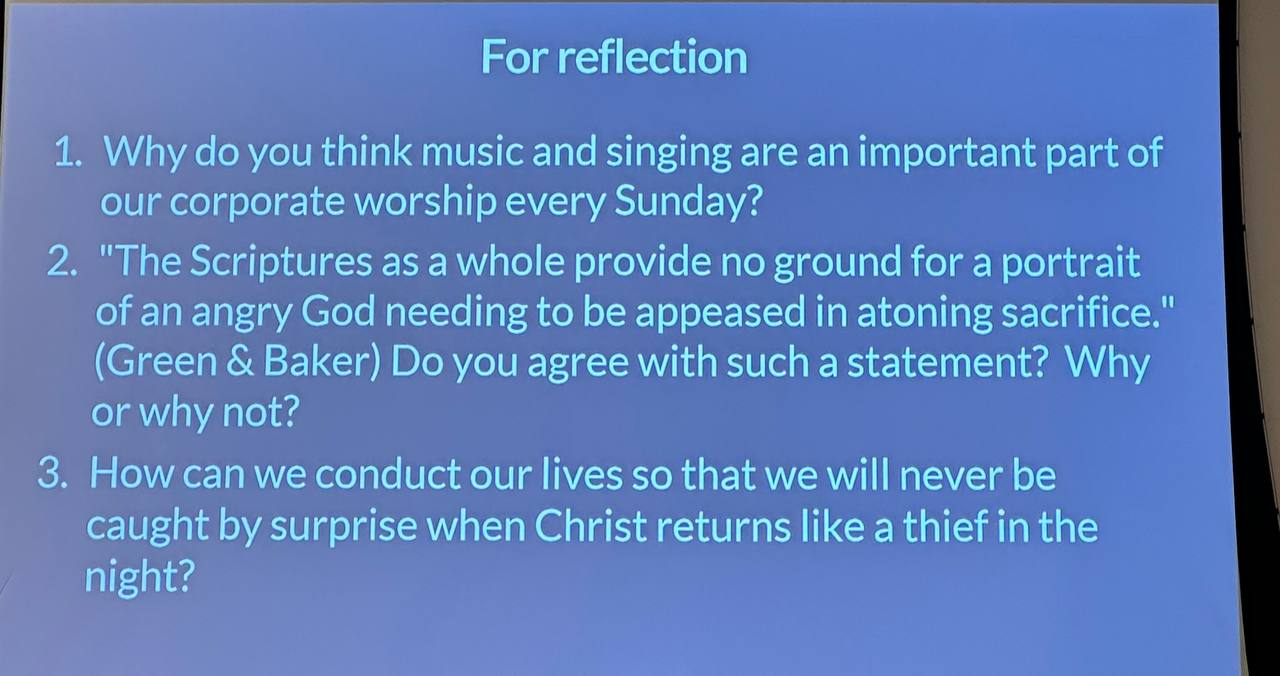
\includegraphics[width=0.8\textwidth, trim={0cm 0cm 0cm 0cm},clip]{Figures/marchSermon4Reflections.jpg}
  %   \includegraphics[width=0.8\textwidth, trim={0cm 0cm 0cm 0cm},clip]{example-image-a}
  %   \caption[]{Reflection questions for this sermon}
  %   \label{}
  % \end{figure}}
\end{itemize}